% THIS IS SIGPROC-SP.TEX - VERSION 3.1
% WORKS WITH V3.2SP OF ACM_PROC_ARTICLE-SP.CLS
% APRIL 2009
%
% It is an example file showing how to use the 'acm_proc_article-sp.cls' V3.2SP
% LaTeX2e document class file for Conference Proceedings submissions.
% ----------------------------------------------------------------------------------------------------------------
% This .tex file (and associated .cls V3.2SP) *DOES NOT* produce:
%       1) The Permission Statement
%       2) The Conference (location) Info information
%       3) The Copyright Line with ACM data
%       4) Page numbering
% ---------------------------------------------------------------------------------------------------------------
% It is an example which *does* use the .bib file (from which the .bbl file
% is produced).
% REMEMBER HOWEVER: After having produced the .bbl file,
% and prior to final submission,
% you need to 'insert'  your .bbl file into your source .tex file so as to provide
% ONE 'self-contained' source file.
%
% Questions regarding SIGS should be sent to
% Adrienne Griscti ---> griscti@acm.org
%
% Questions/suggestions regarding the guidelines, .tex and .cls files, etc. to
% Gerald Murray ---> murray@hq.acm.org
%
% For tracking purposes - this is V3.1SP - APRIL 2009

\documentclass{acm_proc_article-sp}

\usepackage{url}

\begin{document}

\title{Rethinking Scientific Analysis Using \linebreak Modern Scalable Systems}
%
% You need the command \numberofauthors to handle the 'placement
% and alignment' of the authors beneath the title.
%
% For aesthetic reasons, we recommend 'three authors at a time'
% i.e. three 'name/affiliation blocks' be placed beneath the title.
%
% NOTE: You are NOT restricted in how many 'rows' of
% "name/affiliations" may appear. We just ask that you restrict
% the number of 'columns' to three.
%
% Because of the available 'opening page real-estate'
% we ask you to refrain from putting more than six authors
% (two rows with three columns) beneath the article title.
% More than six makes the first-page appear very cluttered indeed.
%
% Use the \alignauthor commands to handle the names
% and affiliations for an 'aesthetic maximum' of six authors.
% Add names, affiliations, addresses for
% the seventh etc. author(s) as the argument for the
% \additionalauthors command.
% These 'additional authors' will be output/set for you
% without further effort on your part as the last section in
% the body of your article BEFORE References or any Appendices.

%  in this sample file, there are a *total*
% of EIGHT authors. SIX appear on the 'first-page' (for formatting
% reasons) and the remaining two appear in the \additionalauthors section.
%
\author{}
% You can go ahead and credit any number of authors here,
% e.g. one 'row of three' or two rows (consisting of one row of three
% and a second row of one, two or three).
%
% The command \alignauthor (no curly braces needed) should
% precede each author name, affiliation/snail-mail address and
% e-mail address. Additionally, tag each line of
% affiliation/address with \affaddr, and tag the
% e-mail address with \email.
%
% 1st. author% There's nothing stopping you putting the seventh, eighth, etc.
% author on the opening page (as the 'third row') but we ask,
% for aesthetic reasons that you place these 'additional authors'
% in the \additional authors block, viz.

% Just remember to make sure that the TOTAL number of authors
% is the number that will appear on the first page PLUS the
% number that will appear in the \additionalauthors section.

\maketitle

\begin{abstract}
Revolutions in data acquisition are drastically changing how science conducts experiments. For
example, ``next-\linebreak generation'' sequencing technologies have driven exponential growth in
the volume of genomic data, and similar trends impact many fields which rely on imaging, such as
astronomy and neuroscience. Although there have been early attempts to use MapReduce systems
to accelerate the processing of these datasets, they have conceded efficiency in favor of using legacy
storage formats and software.

Since the amount of scientific data that is being captured is increasing exponentially, we have a good
opportunity to rethink how we process and store these datasets. In this paper, we introduce a set of
principles for implementing scientific analyses efficiently using commodity ``big data'' systems. We
motivate these principles with an example genomics pipeline which leverages open-source MapReduce
and columnar storage techniques to achieve a $>50\times$ speedup over traditional genomics systems,
at half the cost.
\end{abstract}

% A category with the (minimum) three required fields
\category{L.4.1}{Applied Computing}{Life and medical sciences}[Computational biology]
\category{H.1.3.2}{Information Systems}{Data management systems}[Database management
system engines, parallel and distributed DBMSs]
\category{E.3.2}{Software and its Engineering}{Software creation and management}[Software
Development Process Management]

\terms{Design}

\keywords{Analytics, MapReduce, Genomics, Scientific Computing}

\section{Introduction}
\label{sec:introduction}

With major improvements in scientific data acquisition techniques, data storage and processing have
become major problems for scientists~\cite{schadt10, cunningham14}. In fields like
neuroscience~\cite{freeman14} and genomics~\cite{stein10}, scientists routinely perform experiments
that use terabytes~(TB) to petabytes~(PB) of data. While traditional scientific computing platforms are
optimized for fast linear algebra, many emerging domains make heavy use of statistical learning
techniques coupled with user defined operations on top of semistructured data. This move towards
statistical techniques has been driven by the increase in the amount of data available to scientists, as
well as the rise of statistical systems which are accessible to non-experts, such as
\texttt{Scikit-learn}~\cite{pedregosa11} and \texttt{MLI}~\cite{sparks13}.

While the increase in the amount of scientific data available is a boon for scientists, it puts significant
stress on existing tool chains. Using the current ``best practice'' genomics software~\cite{auwera13}, it
takes approximately 120 hours to process a single, high-quality human genome using a single,
beefy node~\cite{talwalkar14}. To address these challenges, scientists have started to apply computer
systems techniques such as MapReduce~\cite{mckenna10, schatz09, langmead09} and columnar
storage~\cite{fritz11} to custom scientific compute/storage systems. While these systems have improved
the analysis cost and performance, they incur significant overheads due to constraints of the legacy
formats and codebases that they use.

Since the amount of scientific data being generated is growing so quickly, we cannot afford to be
saddled by legacy software and formats. New scientific projects such as the ``100K for UK,'' which aims
to sequence the genomes of 100,000 individuals in the United Kingdom~(UK, \cite{uk100k}) will
generate three to four orders of magnitude more data than prior ``massive'' projects such as the 1000
Genomes Project~\cite{siva08}. While it is important to still be able to use data stored in legacy formats,
the massive amount of \emph{new} data provides us with an opportunity to rethink how we compose
our systems. By choosing the correct mix of computing systems, we can provide better performance and
scalability than custom systems, while enhancing the abstractions exposed to scientists.

In this paper, we demonstrate a system built using Apache Avro, Parquet, and Spark~\cite{avro, parquet,
zaharia10}, which achieves a 50$\times$ increase in throughput over the current best practice pipeline
for processing genomic data. In the process of creating this system, we developed a ``narrow waisted''
layering model for building similar scientific analysis systems. This narrow waisted model is inspired by
the OSI model for networked systems~\cite{zimmermann80}. We then demonstrate the generality of this
model by using it to implement a system for processing astronomy images.

A subtle problem with earlier custom scientific processing and storage systems is that characteristics
of the data format on disk would bleed into the computing model. For example, in the current
Sequence/Binary Alignment and Map~(SAM/BAM~\cite{li09}) formats for storing genomic alignments,
constraints about record ordering are required in order to enable specific computing patterns. We
believe that this is an abstraction inversion, which makes it difficult to perform some other access
patterns. In~\S\ref{sec:principles}, we elucidate why this is a significant problem, and then
in~\S\ref{sec:optimizations-scientific-processing}, we then introduce efficient algorithms for supporting
these computational patterns without forcing constraints on the storage layer.

\section{Background}
\label{sec:background}

As our work exists at the intersection of computational science and data management and processing
systems, our architectural approach is informed by recent trends in both areas. The design of large
scale data management has changed dramatically since the landmark papers by Dean and
Ghemawat~\cite{dean04, dean08} which described Google's \texttt{MapReduce} system. Over a
similar timeframe, scientific fields have moved to take advantage of improvements in data acquisition
technologies. For example, since the Human Genome Project finished in 2001~\cite{lander01}, the price
of genomic sequencing has dropped by 10,000$\times$~\cite{nhgri}. This drop in cost has enabled the
capture of petabytes of sequence data, which has enabled significant population-scale genomics
experiments like the 1000 Genomes project~\cite{siva08}, and The Cancer Genome Atlas~(TCGA,
\cite{weinstein13}). These changes are not unique to genomics; indeed, fields such as
neuroscience~\cite{cunningham14} and astronomy~\cite{turk11} are experiencing similar changes.

There are significant opportunities to apply novel data management systems techniques to scientific
problems. In the rest of this section, we'll look at the current state of the art and opportunities in both
fields.

\subsection{Genomic Data and Analyses}
\label{sec:genomic-data-analyses}

Contemporary genomics has been revolutionized by ``next generation'' sequencing
technologies~(NGS), which have driven a precipitous drop in the cost of running genomic
assays~\cite{nhgri}. Although there are a variety of sequencing technologies in use, the majority of
sequence data comes from the Illumina/Solexa sequencing platform, which uses a
``sequencing-by-synthesis'' technique to generate \emph{short read} data~\cite{metzker09}, where a
sequencing run will generate many reads that are between 50 and 250 bases in length. In addition to
adjusting the length of the reads, we can control the amount of the data that is generated by
changing the amount of the genome that we sequence, or the amount of redundant sequencing that
we perform~(the average number of reads that covers each base, or \emph{coverage}). A single
human genome sequenced at 60$\times$ coverage will produce approximately 1.4 billion reads,
which is approximately 600 GB of raw data, or 225 GB of compressed data. For each read, we also
are provided \emph{quality scores}, which represent the likelihood that the base at a given position
was observed.

One of the most common genomic analyses is \emph{variant calling}, which is a statistical process to
infer the sites at which a single individual varies from the \emph{reference genome}.\footnote{The
reference genome represents the ``average'' genome for a species. The Human Genome
Project~\cite{lander01} assembled the first human reference genome.} This process consists of the
following general steps:

\begin{enumerate}
\item \textbf{Alignment:} For each read, we find the position in the genome that the read is most likely to
have come from. As an exact search is too expensive, there has been an extensive amount of research
which has focused on indexing strategies for improving alignment performance~\cite{li10, li11,
zaharia11}. This process is parallel per sequenced read.
\item \textbf{Pre-processing:} After reads have been aligned to the genome, we perform several
preprocessing steps to eliminate systemic errors in the reads. This may involve recalibrating the
observed quality scores for the bases, or locally optimizing the read alignments. We will present a
description of several of these algorithms in~\S\ref{sec:genomics-pipeline}; for a more detailed
discussion, we refer readers to DePristo et al~\cite{depristo11} and Massie et al~\cite{massie13}.
\item \textbf{Variant calling:} Variant calling is a statistical process which uses the read alignments
and the observed quality scores to compute whether a given sample \linebreak matches or diverges
from the reference genome. This process is typically parallel per position or region in the genome.
\item \textbf{Filtration:} After variants have been called, we want to filter out false positive variant calls.
We may perform queries to look for variants with borderline likelihoods, or we may look for clusters of
variants, which may indicate that a local error has occurred. This process may be parallel per position,
or may involve complex traversals of the genomic coordinate space.
\end{enumerate}

This process is very expensive to run; the current best practice pipeline uses the BWA tool~\cite{li10} for
alignment and the GATK~\cite{mckenna10, depristo11} for pre-processing, variant calling, and filtration.
Current benchmark suites have measured this pipeline as taking between 90 and 130 hours to run
end-to-end~\cite{talwalkar14}. In~\S\ref{sec:genomics-pipeline}, we will demonstrate a distributed
pipeline which achieves a $>50\times$ speedup for the pre-processing component of this pipeline.

\subsection{Scientific Data Processing}
\label{sec:scientific-data-processing}

Although there has been significant progress in the development of systems for processing large
datasets~(e.g., the development of first generation MapReduce systems~\cite{dean04}, followed by
iterative MapReduce systems like Spark~\cite{zaharia10}, as well as parallel and columnar
DBMS~\cite{abadi06, lamb12}), the uptake of these systems in the scientific world has been slow.
Most implementations have either used MapReduce as an inspiration for programming API
design~\cite{mckenna10}, or have been limited systems which have used MapReduce to na\"{i}vely
parallelize existing toolkits~\cite{langmead09, schatz09}. These approaches are perilous for several
reasons:

\begin{itemize}
\item A strong criticism levied against the map-reduce model is that the API is insufficiently expressive
for describing complex tasks. As a consequence of this, tools like the GATK~\cite{mckenna10} which
adopt MapReduce as a programming model~(but \emph{not an execution strategy!!!}) force significant
restrictions on algorithm implementors. For example, a GATK \texttt{walker} is provided with a single
view over the data~(a sorted iterator over a specified region), and is allowed limited reduce functionality.
\item A major contribution of systems like MapReduce~\cite{dean08} and Spark~\cite{zaharia10,
zaharia12} is the ability to reliably distribute parallel tasks across a cluster in an automated fashion. In
practice, to run tools like the GATK across a cluster, organizations have rolled their own systems for
sharding and persisting intermediate data, and managing failures and retries. This is not only an
inefficient duplication of work, but it is also a source of inefficiency during execution: the performance of
iterative stages in the GATK is bottlenecked by I/O performance. Additionally, the sharding techniques
used limit scale-up to a $10\times$ speedup on 23 machines.
\item The na\"{i}ve Hadoop-based implementations in Crossbow~\cite{langmead09} and
Cloudburst~\cite{schatz09} lead to good speedups, but add significant overhead. Several of the
methods that they parallelize incur high overhead due to duplicated loading of indices (for fast aligners,
loading of large indices can be a primary I/O bottleneck) and poor broadcasting of data.
\end{itemize}

A notable exception is the \texttt{Thunder} system, which was developed for processing neuroscience
imaging data~\cite{freeman14}. \texttt{Thunder} performs a largely statistical workload, where clustering
and regression are significant computational tasks. The system is constructed using Spark and Python
and is designed to process datasets larger than 4 TB, and leverages significant functionality from the
MLI/MLLib libraries~\cite{sparks13}.

Recent work by Diao et al~\cite{diao15} has looked at optimizations to MapReduce systems for
processing genomic data. They borrow strategies from the query optimization literature to reorder
computation to minimize data shuffling. While this approach does improve shuffle traffic, several
preprocessing stages cannot be transposed. For instance, reversing the order of indel realignment and
base quality score recalibration~(see~\S\ref{sec:genomics-pipeline}) will change the inferred quality
score distribution. Additionally, we believe that the shuffle traffic that Diao et al observe is an artifact
caused by the abstraction inversion discussed in~\S\ref{sec:introduction}. As we demonstrate
in~\S\ref{sec:genomics-pipeline}, these penalties can be eliminated by restructuring the pre-processing
algorithms.

One interesting trend of note is the development of databases specifically for scientific applications.
The exemplar is SciDB, which provides an array based storage model as well as efficient linear algebra
routines~\cite{brown10}. While arrays accelerate many linear algebra based routines, they are not
a universally great fit. For many genomics workloads, data is semistructured and may consist of strings,
boolean fields, and an array of tagged annotations. Other systems like the Genome Query
Language~\cite{kozanitis14} have extended SQL to provide efficient query semantics across genomic
coordinates. While GQL achieves performance improvements of up to 10$\times$ for certain algorithms,
SQL is not an attractive language for many scientific domains, which make heavy use of user designed
functions~(UDFs), which may be difficult to implement through SQL.

One notable area where database techniques have been leveraged by scientists is in the data storage
layer. Due to the storage costs of large genomic datasets, scientists have introduced the CRAM format
which uses columnar storage techniques and special compression algorithms to achieve a 30\%
reduction in size over the original BAM format~\cite{fritz11}. While CRAM achieves good compression,
it imposes restriction on the ordering and structure of the data, and does not provide support for
predicates or projection. We perform a more comprehensive comparison against CRAM
in~\S\ref{sec:column-store-perf}.

\section{Principles for Scientific \\ Analysis Systems}
\label{sec:principles}

Although there has been significant prior work on scientific computing, most of this work has been
focused on linear algebra and other matrix/network structured problems. 

\subsection{Workloads}
\label{sec:workloads}

Traditionally, work in the scientific computing domain has focused on linear algebra, particle simulations,
and optimization-style problems. The communication and 


\begin{enumerate}
\item Characteristics of data
\begin{enumerate}
\item Scientific data tends to be sparse
\item Different users want to look at different subsets of both rows and columns
\item Data may not always be in a single site, or stored locally
\item \emph{Experimental data} is immutable.
\item What are access patterns?
\end{enumerate}
\item Characteristics of a ideal storage system:
\begin{enumerate}
\item Efficient support for projection of different columns
\item Efficient support for per-record predicates
\item Should not relegate user to a single execution environment
\end{enumerate}
\item Processing:
\begin{enumerate}
\item Workloads are highly variable by field
\item For genomics, workloads are trivially data-parallel
\item Similar for fields with heavy image processing workloads
\item Simulation based fields are tougher; have all-to-all computation pattern, run on supercomputer
\item Defer discussion to~\S\ref{sec:execution-platforms}
\item Ideally, cross-platform.
\end{enumerate}
\end{enumerate}

\subsection{Layering}
\label{sec:layering}

We can improve the efficiency of building scientific data storage and processing systems by choosing
the correct abstractions. 

The BAM and VCF formats are difficult to specialize for certain processing patterns without changing the
implementation of the formats themselves. This issue is similar to the problems addressed during the
development of the Open Systems Interconnection~(OSI) model and Internet Protocol~(IP) stack for
networking services~\cite{zimmermann80}. The developers  of the OSI model and the IP stack needed
to make many different technologies and systems function in unison---to do this, they introduced the
concept of a ``narrow waist,'' which guaranteed that a new protocol or technology would be compatible
with the rest of the system if it implemented one specific interface.

We draw inspiration from the development of networking standards---we believe that our largest
contribution is the explicit ADAM schema, which is the ``narrow waist'' in our stack. This schema allows
components to be cleanly interchanged as long as they implement the ADAM schema.
Figure~\ref{fig:stack-model} shows our stack.

\begin{figure}[h]
\begin{center}
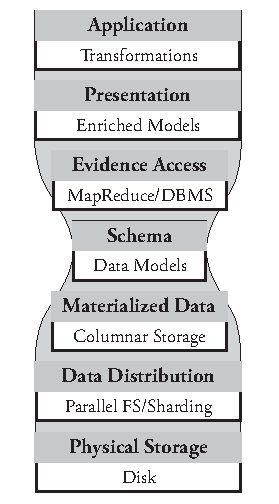
\includegraphics[width=0.6\linewidth]{stack-model.pdf}
\end{center}
\caption{A Stack Model for Genomics}
\label{fig:stack-model}
\end{figure}

The seven layers of our stack model are decomposed as follows, traditionally numbered from bottom to
top:

\begin{enumerate}
\item {\bf Physical Storage:} This layer coordinates data writes to physical media, usually magnetic disk.
\item {\bf Data Distribution:} This layer manages access, replication, and distribution of the genomics
files that have been written to disk.
\item {\bf Materialized Data:} This layer encodes the patterns for how data is encoded and stored. This
provides read/write efficiency
and compression.
\item {\bf Data Schema:} This layer specifies the representation of data when it is accessed, and forms
the narrow waist of the pipeline.
\item {\bf Evidence Access:} This layer implements efficient methods for performing common access
patterns such as random database
queries, or sequential/parallel reading of records from a flat file.
\item {\bf Presentation:} The presentation layer provides the application developer with efficient and
straightforward methods for querying the characteristics of individual portions of genetic data.
\item {\bf Application:} Applications like variant calling and alignment are implemented in this layer.
\end{enumerate}

The ADAM schema is represented using Apache Avro~\cite{avro}, an open-source, cross-platform data
serialization framework similar to Apache Thrift and Google's Protocol Buffers~\cite{thrift, protobuf}.
Avro was chosen as the interchange format for several reasons:

\begin{itemize}
\item Avro is an open-source framework covered by the Apache 2 license, which means that Avro can be
used with both open and closed source software.
\item Avro has broad cross-platform support. Natively, Avro supports C/C++/C\#, Java, Scala, Python,
Ruby, and php.
\item Avro provides a clear and human readable language for explicitly describing the schema of an
object~(Avro Description Language, AVDL).
\item Avro is natively supported by several common Map-Reduce frameworks and database systems.
\item Avro schemas can be updated without breaking compatibility with objects written using a previous
version of the schema.
\end{itemize}

For a system to implement the ADAM format, it must read/write ADAM objects that are defined by Avro
schemas. As such the schemas provide the common ground for tools to interoperate, thereby allowing
the user to interchange one tool for another and minimize tool or vendor lock-in.

A well defined software stack has several other significant advantages. By limiting application
interactions with layers lower than the presentation layer, application developers are given a clear and
consistent view of the data they are processing, and this view of the data is independent of whether the
data is local or distributed across a cluster or cloud. By separating the API from the data access layer,
we improve flexibility. With careful design in the data format and data access layers, we can seamlessly
support conventional flat file access patterns, while also allowing easy access to data with database
methods. By treating the compute substrate and storage as separate layers, we also drastically increase
the portability of the APIs that we implement.

Talk about data storage bleeding into programming model.

We need to:

\begin{enumerate}
\item Show how current systems fit into the stack model, and how our proposed stack is different
\item Elucidate why it is more efficient to build systems that are decomposed as per our stack above
(reference networking stack and protocol interchange), see Bafna et al~\cite{bafna13}, talk about costs
of programming without good stack model
\end{enumerate}

\section{Case Studies}
\label{sec:case-studies}

To validate our architectural choices, we have implemented pipelines for processing short read genomic
data and astronomy image processing. Both of these pipelines are implemented using
Spark~\cite{zaharia10}, Avro~\cite{avro}, and Parquet~\cite{parquet}. We have chosen these two
applications as they fit in different areas in the design space. 

\subsection{Genomics Pipeline}
\label{sec:genomics-pipeline}

\paragraph{Sorting}
\label{sec:sorting}
This phase sorts all reads by the position of the start of their alignment. The implementation of this
algorithm is trivial, as Spark provides a sort primitive~\cite{zaharia10}; we solely need to define an
ordering for genomic coordinates, which is well defined.

\paragraph{Duplicate Removal} 
\label{sec:duplicate-removal}
During the process of preparing DNA for sequencing, errors in the sample preparation and polymerase
chain reaction~(PCR) stages can cause the duplication of reads. Detection of duplicate reads requires
matching all reads by their position and orientation after read alignment. Reads with identical position
and orientation are assumed to be duplicates. When a group of duplicate reads is found, each read is
scored, and all but the top-scoring read are marked as duplicates.

\paragraph{Base Quality Score Recalibration} 
\label{sec:bqsr}
During the sequencing process, systemic errors occur that lead to the incorrect assignment of base
quality scores. In this step, we build a statistical model for read errors

\paragraph{Local Realignment} 
\label{sec:local-realignment}
For performance reasons, all modern aligners use algorithms that provide approximate alignments. This approximation can cause reads with
evidence of indels to have slight misalignments with the reference. In this stage, we use fully accurate sequence alignment
methods~(Smith-Waterman algorithm~\cite{smith81}) to locally realign reads that contain evidence of short indels. This pipeline
step is omitted in some variant calling pipelines if the variant calling algorithm used is not susceptible to these
local alignment errors.

For current implementations of these read processing steps, performance is limited by disk bandwidth. This bottleneck occurs  because the operations
read in a SAM/BAM file, perform a bit of processing, and write the data to disk as a new SAM/BAM file. We address this problem by performing
our processing iteratively in memory. The four read processing stages can then be chained together, eliminating three long writes to
disk and an additional three long reads from disk. The stages themselves cannot be performed in parallel, but the operations inside each
stage are data parallel. 

\subsection{Astronomy Image Processing}
\label{sec:astronomy-image-processing}
The Montage~\cite{montage} application is a typical astronomy image processing pipeline that builds mosaics from small image 
tiles obtained from telescopes with the requirement of preserving the energy quantity and position for each pixel between the 
input and output images. The pipeline has multiple stages that can be grouped into the following phases.

\paragraph{Tile Reprojection}
The raw input images are reprojected with the defined scale as required in the final mosaic. 

\paragraph{Background Modeling}
This phase smoothes out the background levels between each pair of overlapped images and fits a plane to each of them. The phase can be further divided into steps of overlap calculation, difference image creation, and plane-fitting coefficient calculation.

\paragraph{Background Matching}
The background matching phase applies background removal to the reprojected images with the best solution derived from previous phase to smooth out the overlap regions.

\paragraph{Tile Mosaicing}
The tile masoning phase coadds all corrected images (after applying background matching to the reprojected images) into a aggregated mosaic file. This phase also involves a metadata processing stage before the mosaicing.

The tile reproduction, background modeling, and background matching phases are embarrassingly parallel, with each task (both computation and I/O) running independent from other tasks in the same phase. The tile mosaicing phase aligns the tiles of the matrix and applies a function (the function can be average, median, or count) to the overlapped pixels. All functions can be applied to the overlapped pixels in an embarrassingly parallel manner, while the I/O are done through a single process.

We care specifically about the tile mosaicing phase as the current implementation requires a preceding stage to summarize the metadata of all corrected images to produce a metadata table containing the tile positioning information. This particular stage has to read all input files into memory, but only accesses a small portion of the file. Also the current implementation parallelize the computation with each matrix row as the element, which results in inefficient input images replication when executed in a distributed environment. We address the first by explicitly declaring the image data schema and storing the images in a column store, so that all input images can be loaded to memory just once with all subsequent computation in memory. The metadata processing can access data that is continuous on a disk, while the rest of the I/O can be done in parallel.

\section{Data Access Optimizations for \\ Scientific Processing}
\label{sec:optimizations-scientific-processing}

\subsection{Coordinate System Joins}
\label{sec:coordinate-system-joins}

This will be a compare/contrast discussion of the multiple join algorithms we've created. TBD.

\subsection{Loading Remote Data}
\label{sec:loading-remote-data}

\begin{enumerate}
\item Data may not be kept locally
\begin{enumerate}
\item Too much data to keep locally
\item Not all data is hot
\end{enumerate}
\item May push data off local disks into block store
\item Manually re-staging data has high latency cost $\rightarrow$ impacts throughput
\item What do we need to do to accommodate this?
\begin{enumerate}
\item Efficient indexing
\item Remote push-down predicate
\end{enumerate}
\item Discuss S3/Parquet interaction
\end{enumerate}

\section{Performance}
\label{sec:performance}


\subsection{Genomics Workloads}
\label{sec:genomics-performance}

Table~\ref{tab:overview} previews the performance of ADAM for \textit{Sort}, \textit{Mark Duplicates},
and \textit{Flagstat}. The tests in this table are run on the high coverage \textit{NA12878} full genome
BAM file that is available from the 1000 Genomes project; the HG00096 low coverage BAM from 1000
Genomes is used later in this section\footnote{The files used for these experiments can be found on the
1000 Genomes ftp site, \url{ftp.1000genomes.ebi.ac.uk} in directory
\texttt{/vol1/ftp/data/NA12878/high\_coverage\_alignment/} for NA12878, and in directory
\texttt{/vol1/ftp/data/HG00096/alignment/} for HG00096.}. These tests have been run on the EC2 cloud,
using the instance types listed. We compute the cost of running each experiment by multiplying the
number of instances used by the total wall time for the run and by the cost of running a single instance
of that type for an hour, which is the process Amazon uses to charge customers.

\begin{table}[h]
\caption{\textit{Sort}, \textit{Mark Duplicates}, and \textit{Flagstat} Performance on NA12878}
\label{tab:overview}
\begin{tabular}{ l c c c c }
\hline
\multicolumn{5}{c}{\bf \textit{Sort}} \\
\bf Software & \bf EC2 profile & \bf Wall Time & \bf Speedup & \bf Cost \\
\hline
Picard 1.103 & 1 \texttt{hs1.8xlarge} & 17h 44m & 1$\times$ & \$81.57 \\
ADAM 0.5.0 & 1 \texttt{hs1.8xlarge} & 8h 56m & 2$\times$ & \$41.09 \\
ADAM 0.5.0 & 32 \texttt{cr1.8xlarge} & 33m & 32$\times$ & \$61.60 \\
ADAM 0.5.0 & 100 \texttt{m2.4xlarge} & 21m & 52$\times$ & \$56.00 \\ 
\hline
\multicolumn{5}{c}{\bf \textit{Mark Duplicates}} \\
\bf Software & \bf EC2 profile & \bf Wall Time & \bf Speedup & \bf Cost  \\
\hline
Picard 1.103 & 1 \texttt{hs1.8xlarge} & 20h 22m & 1$\times$ & \$93.68 \\
ADAM 0.5.0 & 100 \texttt{m2.4xlarge} & 29m & 42$\times$ & \$79.26 \\
\hline
\multicolumn{5}{c}{\bf \textit{Flagstat}} \\
\bf Software & \bf EC2 profile & \bf Wall Time & \bf Speedup & \bf Cost  \\
\hline
SAMtools 0.1.19 & 1 \texttt{hs1.8xlarge} & 25m 24s & 1$\times$ & \$1.95 \\
ADAM 0.5.0 & 32 \texttt{cr1.8xlarge} & 0m 46s & 33$\times$ & \$1.43 \\
\hline
\end{tabular}
\end{table}

Table~\ref{tab:machines} describes the instance types. Memory capacity is reported in Gibibytes~(GiB),
where 1 GiB is equal to $2^{30}$ bytes. Storage capacities are not reported in this table because disk
capacity does not impact performance, but the number and type of storage drives is reported because
aggregate disk bandwidth does impact performance. In our tests, the \texttt{hs1.8xlarge} instance is
chosen to represent a workstation. Network bandwidth is constant across all instances.

\begin{table}[h]
\caption{AWS Machine Types}
\label{tab:machines}
\begin{tabular}{ l c l }
\hline
\bf Machine & \bf Cost & \bf Description \\
\hline
\hline
\texttt{hs1.8xlarge} & \$4.60/hr/machine & 16 cores, 117GiB RAM, 24$\times$ HDD \\
\texttt{cr1.8xlarge} & \$3.50/hr/machine & 32 cores, 244GiB RAM, 2$\times$ SDD \\
\texttt{m2.4xlarge} & \$1.64/hr/machine & 8 cores, 68.4GiB RAM, 2$\times$ HDD \\
\hline
\end{tabular}
\end{table}

As can be seen from these results, the ADAM pipeline is approximately twice as fast as current pipelines
when running on a single node. Additionally, ADAM achieves speedup that is close to linear. This point is
not clear from Table~\ref{tab:overview}, as we change instance types when also changing the number of
instances used. To clarify, Figure~\ref{fig:speedup} presents speedup plots for the NA12878 high
coverage genome and the HG00096 low coverage genome~(16 GB BAM). These speedup
measurements are taken on a dedicated cluster of 82 machines where each machine has 24 Xeon
cores, 128GB of RAM, and 12 disks.

\begin{figure}[h]
\begin{center}
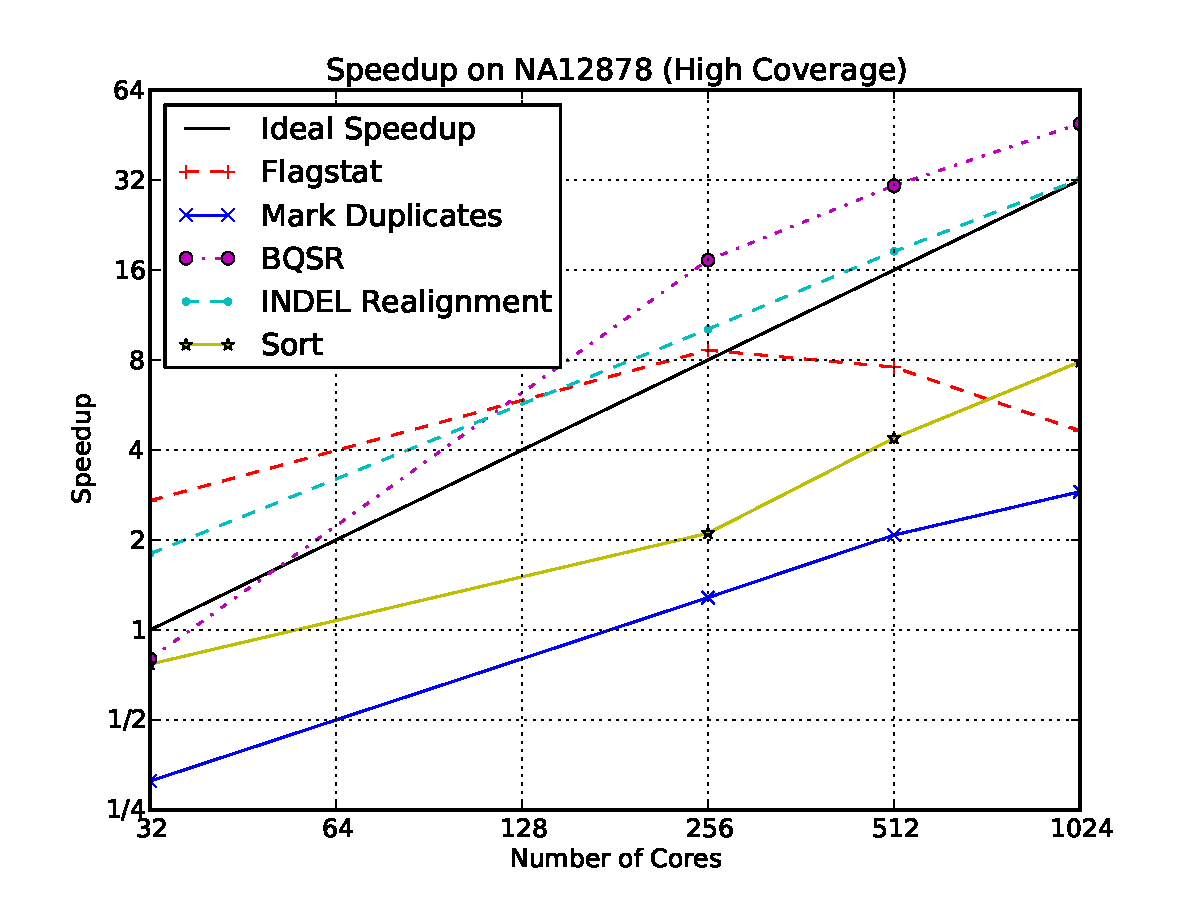
\includegraphics[width=0.99\linewidth]{graphs/speedup_na12878.pdf}
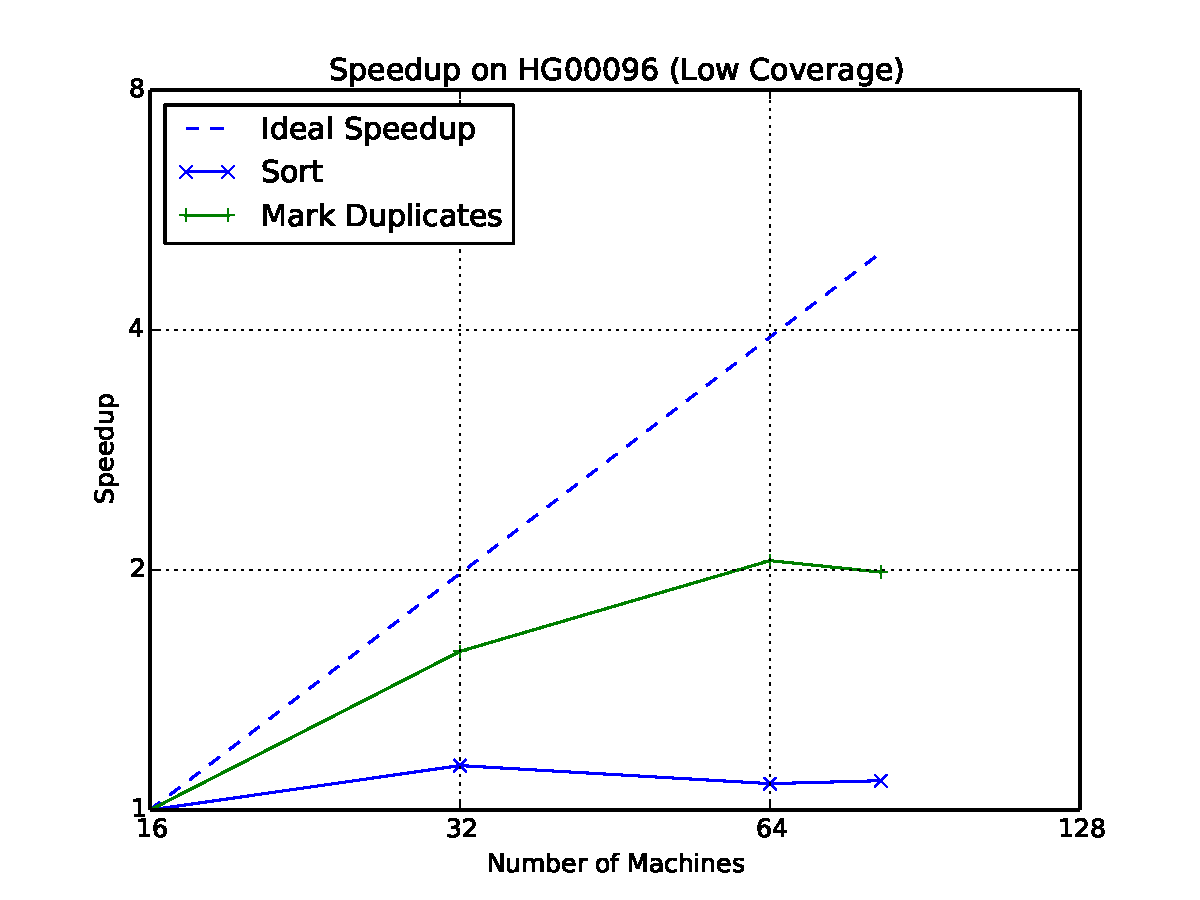
\includegraphics[width=0.99\linewidth]{graphs/speedup_hg00096.pdf}
\end{center}
\caption{Speedup when running \textit{Sort} and \textit{Mark Duplicates} on NA12878 and HG00096}
\label{fig:speedup}
\end{figure}

NA12878 sees linear speedup for both \textit{Sort} and \textit{Mark Duplicates} through 82 nodes. With
82 nodes, it takes 8.8 minutes to sort reads, and 14 minutes to mark duplicate reads across the 250GB
file. HG00096 is a significantly smaller genome at 16 GB. Although the speedup from sorting diminishes
after 16 nodes, duplicate marking sees speedup through 64 nodes. With HG00096 on 64 nodes, each
machine in the cluster is responsible for processing only 250MB of data. Sorting completes in 3.3
minutes, and duplicate marking completes in 2.3 minutes. The speedup is limited by several factors:

\begin{itemize}
\item Although columnar stores have very high read performance, they are limited by write performance.
Our tests exaggerate this penalty---as a variant calling pipeline will consume a large read file, but then
output a variant call file that is approximately two orders of magnitude smaller, the write penalty will be
reduced.
\item Additionally, for large clusters, straggler elimination is an issue. Phases of both \textit{Sort} and
\textit{MarkDuplicates} currently suffer from stragglers---we are in the process of addressing these
issues.
\end{itemize}

However, as noted above, speedup continues until we reach approximately 1GB of data per node for
sorting, or 250MB of data per node for duplicate marking. For a high coverage whole genome like
NA12878, this should theoretically allow speedup through 250 nodes for sorting and 1,000 nodes for
duplicate marking.

\subsection{Astronomy Workloads}
\label{sec:astro-workloads}
We use the 2MASS data and the Montage test case of 3x3 degree mosaicing with Galaxy m101 as the center. 
The tile mosaicing phase has 1.5GB input data and produces a 2.7GB aggregated output file.

\subsection{Column Store Performance}
\label{sec:column-store-perf}

Compare to CRAM.

\section{Discussion}
\label{sec:discussion}


\subsection{Evolution of Computing Infrastructure}
\label{sec:evolution-computing-infrastructure}

% I use a cluster everday, you must be more specific here, more generally, I think you are losing the main point here. You don't need a pitch for cloud computing here. Instead is the point that you really want to make that the cloud makes it more difficult to implement traditional shared memory clusters.
As traditional genomics workflows could not easily or efficiently use compute clusters, many users have
performed the bulk of their processing on beefy workstations. We predict that the rise of distributed
computing tools for genomics will soon render workstations unattractive. Instead, we expect that
clinical/research centers will either process consistently high volumes of genomic data and build and
maintain their own dedicated compute farms, or will use a cloud computing platform for infrequent data
processing needs. The benefits of cloud computing include:

\begin{itemize}
\item Commercial cloud platforms are economically attractive as they do not present capital acquisition
costs, nor do they have maintenance costs.
\item Additionally, cloud platforms tend to offer several levels of service differentiation. Users can trade
cost for performance, as the number of machines and performance of machines can be selected.
Additionally, cloud platforms also frequently auction unused slots off at below-market
prices~(\emph{spot instances}, which can further reduce costs.
\item System setup can be simplified through the use of systems like \texttt{Docker}~\cite{docker} for
distributing consistent application images.
\item Inexpensive pay-as-you-go storage solutions are available which provide good performance when
used with a cloud service.
\end{itemize}

We anticipate that our design decisions will make the transition to cloud services for scientific data
systems more attractive.

We anticipate that formats like ADAM will ease this transition, as ADAM can be used efficiently on all
platforms. Additionally, ADAM's stack model explicitly allows for significant flexibility in the format, which
will allow ADAM to easily adapt to future computing innovations.

\subsection{Syntax vs. Semantics}
\label{sec:syntax-vs-semantics}

When selecting a storage format, it is important to address both the problems of syntax and semantics.
A storage backend that is \emph{syntactically good} will be easily adaptable to multiple platforms,
provide good programming abstractions and APIs, and will be performant. A format that is
\emph{semantically good} will provide data representations that closely mirror the scientific and
algorithmic processes they represent.

The core of the ADAM project is focused on improving the syntax used for representing biological data.
Our focus on semantics is limited to introducing semantic improvements for variant and genotype data
that allows for better representation of joint called data and annotations~\S\ref{sec:adamvariant}.
However, while we do not address the greater issues of semantics, we provide a clean platform for
tacking these issues because of the ADAM stack and its ability to support broader access and
computational patterns. For example, ADAM data can easily be accessed using databases like
Spark-SQL and Impala. Additionally, ADAM can be used as the base of a graph-based data
representation through GraphX~\cite{xin13}. This design decision allows for the easy and clean
extension of ADAM's semantics.

\subsection{Advantages of Commodity Systems}
\label{sec:commodity}

In~\S\ref{sec:layering}, we advocate for a cleanly decomposed system. In our case studies
in~\S\ref{sec:case-studies}, we then used the open source Avro, Parquet, and Spark systems to
implement our stack~\cite{avro, parquet, zaharia10}. An obvious advantage of using commodity
systems is code reuse, but the benefits do not start and end there. By using components that are well
accepted in the Hadoop ecosystem, we gain several major features for free:

\begin{enumerate}
\item Beyond efficient parallel performance, Parquet is also supported as a data format by several
database-like systems, like Spark-SQL and Impala. This allows us to support efficient database style
processing, without needing to manually retrofit a tool like GQL to the data~\cite{kozanitis14}.
\item While the native Spark Scala API provides rich programming abstractions, scientists may prefer
other language environments, like Python or R. Other scientific systems like SciDB~\cite{brown10}
support native Python and R bindings. Likewise, we provide distributed processing using Python
through PySpark.
\end{enumerate}

\subsection{Non-Data Parallel Scientific Computing}
\label{sec:ndp-sci}

\section{Conclusion}
\label{sec:conclusion}

In the end, we conclude.

\appendix

\bibliographystyle{abbrv}
\bibliography{adam} 

%\balancecolumns
% That's all folks!
\end{document}
